\documentclass[10pt]{exam}
\usepackage[T1]{fontenc}
\usepackage[paper=a4paper,margin=2cm]{geometry}
\usepackage[sfdefault,light]{roboto}

\usepackage[usenames,dvipsnames]{xcolor}
\usepackage{amsmath,amssymb,array,graphicx,enumitem,listings,lstautogobble,multicol,textcomp,titlesec}
\usepackage{mathtools}

\setlength\parindent{0cm}

%Title & Section Formatting
\titleformat{\section}{\normalfont\Large\bfseries}{}{0em}{}[{\titlerule[0.5pt]}]
\titleformat{\subsection}{\normalfont\large\bfseries}{}{0em}{}

%Mathematical Shortcuts
\newcommand{\floor}[1]{\left\lfloor #1 \right\rfloor}
\newcommand{\ceil}[1]{\left\lceil #1 \right\rceil}

%Listings Shortcuts & Settings
\newcommand{\code}[1]{\lstinline{#1}}
\lstset{language=Java,
        autogobble=true,
        basicstyle=\ttfamily,
        commentstyle=\color{black!45},
        keywordstyle=\bfseries,
        showstringspaces=false,
        upquote=true}

%General Shortcuts
\newcommand{\blankpage}{\null\thispagestyle{empty}\addtocounter{page}{-1}\newpage}

\usepackage{draftwatermark,transparent}
\SetWatermarkAngle{0}
\SetWatermarkText{\transparent{0.025}\includegraphics[scale=0.75]{graphics/logo_black.png}}

%Color-Coded questions
\newcommand{\ColourQuestion}[3]{\renewcommand{\questionlabel}{\colorbox{#1}{\bfseries\color{white}\thequestion}\hfill}\question[#3] #2}
\newcommand{\BlueQuestion}[1]{\ColourQuestion{RoyalBlue}{#1}{1}}
\newcommand{\GreenQuestion}[1]{\ColourQuestion{ForestGreen}{#1}{2}}
\newcommand{\YellowQuestion}[1]{\ColourQuestion{Goldenrod}{#1}{4}}
\newcommand{\RedQuestion}[1]{\ColourQuestion{BrickRed}{#1}{6}}
\newcommand{\PurpleQuestion}[1]{\ColourQuestion{RoyalPurple}{#1}{30}}
\pointsinrightmargin

\header{\footnotesize\scshape Assignment \#\AssignmentNumber: \AssignmentTitle}{}{}
\cfoot{\footnotesize\scshape \AssignmentCourse\\Woodstock School---Mussoorie, Uttarakhand---India}

\usepackage[hang,flushmargin]{footmisc}
\renewcommand{\thefootnote}{\fnsymbol{footnote}}

\def\AssignmentCourse{AP Computer Science Principles}
\def\AssignmentNumber{04}
\def\AssignmentTitle{Conditionals}

\begin{document}
  \begin{questions}
    %Error detection/fix?
    \BlueQuestion{Explain what, if anything, is wrong with each of the following code fragments. You may assume all variables are initialized appropriately.}
      \begin{parts}
        \part 
          \begin{lstlisting}
            if (a = 4) {
              ellipse(50, 50, 100, 100);
            }
          \end{lstlisting}
          
        \part
          \begin{lstlisting}
            if (a == 10); {
              ellipse(50, 50, 100, 100);
            }
          \end{lstlisting}

        \part
          \begin{lstlisting}
            if (a == 20)
              ellipse(50, 50, 100, 100);
          \end{lstlisting}
      \end{parts}

    \BlueQuestion{Processing, and many other programming languages, have separate operators for comparing the equality of two values (\code{==}) and for assigning a value to a variable (\code{=}). Briefly discuss the pros and cons of having different operators for these operations.}

    %Heads / Tails
    \GreenQuestion{Write a program that will simulate a random coin toss using Processing's \code{random()} method and display a coin representing either ``heads'' or ``tails''. Run your program multiple times to ensure it is working as intended.}
      \begin{center}
        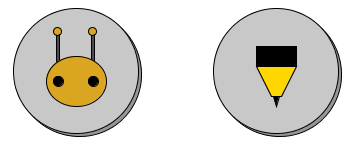
\includegraphics[scale=0.5]{files/Coins}
      \end{center}

    \GreenQuestion{Write a program that will generate $4$ circles of random diameters ranging from $0$ to $150$ with the following colour requirements:}
      \begin{parts}
        \part if the diameter of the circle is less than $50$, the circle should be coloured \emph{blue},
        \part if the diameter of the circle is between $50$ and $100$ (inclusive), the circle should be coloured \emph{green}, and
        \part if the diameter of the circle is greater than $100$, the circle should be coloured \emph{red}.
      \end{parts}
      Run your program multiple times to ensure it is working as intended.

    %HSB/RGB
    \RedQuestion{The RGB colour model is not the only model used to express different colours in a computer system. Processing also allows us to express colours in a model known as \textbf{H}ue, \textbf{S}aturation, and \textbf{B}rightness (HSB), also sometimes referred to as Hue/Saturation/Value (HSV). Because HSB can be used to express the exact same set of colours as RGB, there is a method for converting between the two. That is, given values for $R$ed, $G$reen, and $B$lue, you can derive $H$ue, $S$aturation, and $Br$ightness using the following algorithm\footnote[2]{This algorithm is adapted from the RapidTables RGB to HSV conversion algorithm found at: http://www.rapidtables.com/convert/color/rgb-to-hsv.htm.}.}
      {\footnotesize
      \begin{center}
        \fcolorbox{black}{black!15}{\parbox{0.9\textwidth}{
          \textbf{To Calculate Hue:}
          \begin{enumerate}
            \item First, calculate $Rp$, $Gp$, and $Bp$ such that:
              \[\begin{aligned}
                Rp &= R \div 255\\
                Gp &= G \div 255\\
                Bp &= B \div 255
              \end{aligned}\]
            \item Next, calculate $max$, $min$, and $d$ as:
              \[\begin{aligned}
                max &= max(Rp, Gp, Bp)\\
                min &= min(Rp, Gp, Bp)\\
                d &= max - min
              \end{aligned}\]
            \item Finally, calculate $H$ using the following piecewise function:
              \[
                H = \left\{\begin{array}{l r}
                  0, & d = 0\\
                  60 \times \left(\frac{Gp - Bp}{d} \mathbf{\ mod\ } 6\right), & max = Rp\\
                  60 \times \left(\frac{Bp - Rp}{d} + 2\right), & max = Gp\\
                  60 \times \left(\frac{Rp - Gp}{d} + 4\right), & max = Bp
                \end{array}\right.
              \]
          \end{enumerate}
        }}
      \end{center}
      \begin{center}
        \fcolorbox{black}{black!15}{\parbox{0.9\textwidth}{        
          \textbf{To Calculate Saturation:}

            Calculate $S$ using the following piecewise function:
            \[
              S = \left\{\begin{array}{l r}
                0, & max = 0\\
                \frac{d}{max}, & max \ne 0
              \end{array}\right.
            \]
        }}
      \end{center}
      \begin{center}
        \fcolorbox{black}{black!15}{\parbox{0.9\textwidth}{
          \textbf{To Calculate Brightness:}

            The brightness is always equal to the highest of $Rp$, $Gp$, and $Bp$. That is,
            \[
              Br = max
            \]
        }}
      \end{center}
      \begin{center}
        \parbox{0.9\textwidth}{\textbf{Note:} This will result in an $H$ value between $0$ and $360$ and $S$ and $Br$ values between $0$ and $1$. Processing allows us to switch to this colour model using its \code{colorMode()} method. In particular, to switch to the values generated using the above algorithm, we can call: \code{colorMode(HSB, 360, 1, 1)}.
        }
      \end{center}
      }

      Write a program that initializes values for \code{R}, \code{G}, and \code{B} and uses the above algorithm to calculate \code{H}, \code{S}, and \code{Br}. Test your program by displaying two squares, side-by-side, the first using a \code{fill()} in RGB and the second using a \code{fill()} in HSB (after having set the \code{colorMode()}).
      \begin{center}
        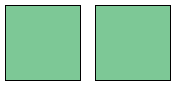
\includegraphics[scale=0.5]{files/Squares}
      \end{center}
      {\small\textbf{Note:} Vary R, G, and B between runnings of your program in order to ensure H, S, and Br are being calculated correctly.}
    %Complementary Colors
    \YellowQuestion{\emph{Complementary colours} are colours that appear on opposite sides of the colour wheel. Although the colour wheel was first developed by artists using primary pigment colours (red, blue, and yellow), we can still find a colour complementary to one using the RGB model. In order to do so, it is important to note that the range of \emph{hue} values in the HSB model being $0$--$360$ is no coincidence: hue actually refers to the angle around the colour wheel at which the particular colour appears. The algorithm for finding an RGB modelled colour's complement, therefore, is:}
      {\footnotesize
      \begin{center}
        \fcolorbox{black}{black!15}{\parbox{0.9\textwidth}{
          \textbf{To Find an RGB Complement:}

          \begin{enumerate}
            \item Convert from RGB to HSB.
            \item Calculate $H = (H + 180) \mathbf{\ mod\ } 360$.
            \item Convert from HSB to RGB.
          \end{enumerate}
        }}
      \end{center}
      \begin{center}
        \parbox{0.9\textwidth}{
          {\textbf{Note:} Because Processing allows us to draw in HSB colour mode, the last step of the algorithm is not strictly required and is not part of this assigment.}
        }
      \end{center}
      }

      \begin{parts}
        \part Write a program that initializes values for \code{R}, \code{G}, and \code{B} and uses the above algorithm (omitting Step \#3) to find the colour's complement. Test your program by displaying two squares, side-by-side, the first using a \code{fill()} of the original colour and the second using a \code{fill()} of its complement. Make sure you switch to the HSB \code{colorMode()} before drawing the second square.\\
        {\small\textbf{Hint:} Use your RGB to HSB program from Question \#5.}
        \part Explain why adding $180$ to $H$ in the HSB value finds a colour on the opposite side of the colour wheel.
        \part Explain why the new $H$ value needs to be taken $\mathbf{mod\ } 360$.
      \end{parts}
  \end{questions}
\end{document}
